\documentclass[tikz,border=2pt]{standalone}
\renewcommand{\familydefault}{\sfdefault}
\usetikzlibrary{arrows.meta,calc,positioning}
\tikzset{every picture/.style={line width=1pt, >=Stealth},
         hl/.style={fill=black, fill opacity=0.12, text opacity=1}}
\begin{document}
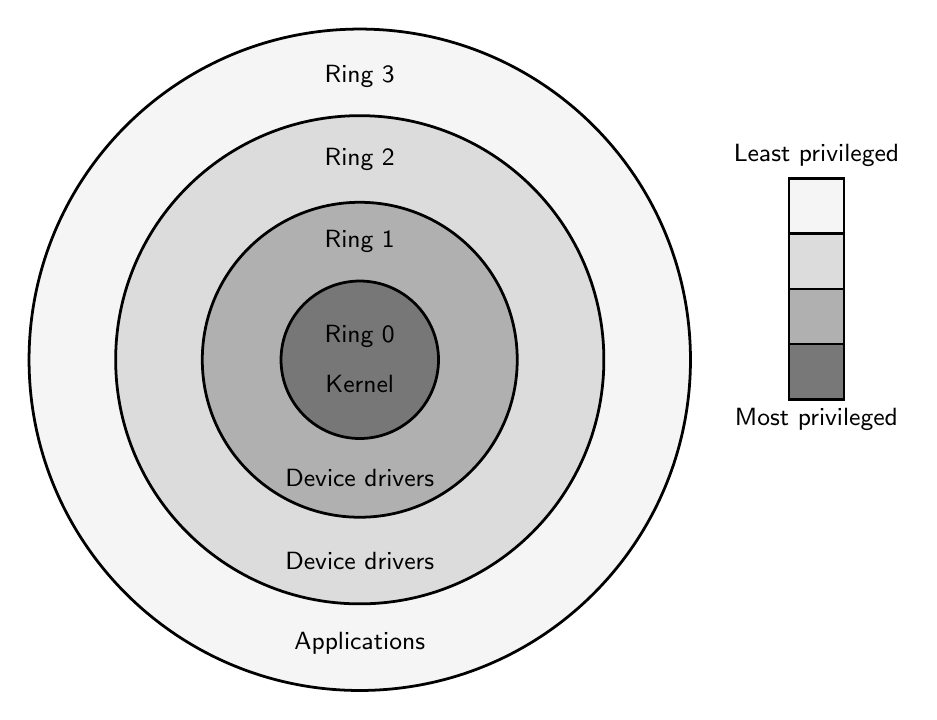
\begin{tikzpicture}
  % Darker rings are more privileged.
  \foreach \r/\o in {4.2/0.04, 3.1/0.1, 2/0.2, 1/0.32} \draw[fill=black, fill opacity=\o] (0, 0) circle (\r);
  \foreach \y/\ring/\who in {3.6/3/Applications, 2.55/2/Device drivers, 1.5/1/Device drivers, 0.3/0/Kernel} {
    \node[font=\small] at (0, \y) {Ring \ring};
    \node[font=\small] at (0, -\y) {\who};
  }
  % Legend
  \node[font=\small] at (5.8, 2.6) {Least privileged};
  % Each swatch uses the combined opacity of the nested circles over that ring.
  \foreach \o [count=\k] in {0.04, 0.136, 0.309, 0.53} \draw[fill=black, fill opacity=\o] (5.45, 2.3 - 0.7*\k) rectangle ++(0.7, 0.7);
  \node[font=\small] at (5.8, -0.75) {Most privileged};
\end{tikzpicture}
\end{document}
